\documentclass{article}
\usepackage{tikz}
\usetikzlibrary{arrows.meta,positioning,calc,shapes.geometric}
\pagestyle{empty}
\begin{document}
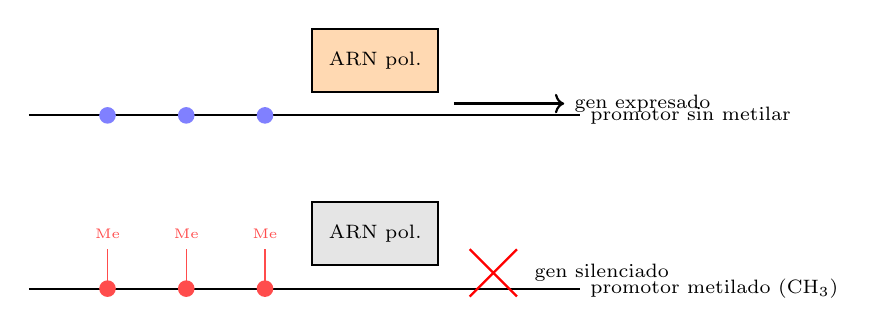
\begin{tikzpicture}

\draw[thick] (0,2.6) -- (7,2.6) node[right, font=\scriptsize] {promotor sin metilar};
\foreach \x in {1.0,2.0,3.0} {\fill[blue!50] (\x,2.6) circle (3pt);}
\draw[thick, fill=orange!30] (3.6,2.9) rectangle (5.2,3.7); \node[font=\scriptsize] at (4.4,3.3) {ARN pol.};
\draw[->, thick] (5.4,2.75) -- (6.8,2.75) node[right, font=\scriptsize] {gen expresado};
\draw[thick] (0,0.4) -- (7,0.4) node[right, font=\scriptsize] {promotor metilado (CH$_3$)};
\foreach \x in {1.0,2.0,3.0} {\fill[red!70] (\x,0.4) circle (3pt); \draw[red!70] (\x,0.4) -- (\x,0.9); \node[font=\tiny, red!70] at (\x,1.1) {Me};}
\draw[thick, fill=gray!20] (3.6,0.7) rectangle (5.2,1.5); \node[font=\scriptsize] at (4.4,1.1) {ARN pol.};
\draw[thick, red] (5.6,0.3) -- (6.2,0.9) (5.6,0.9) -- (6.2,0.3); \node[font=\scriptsize, right] at (6.3,0.6) {gen silenciado};

\end{tikzpicture}
\end{document}
